


% --------------


%Étape 1 : Algorithme de Déplacement Autonome


%Sommaire 
%Introduction	3


\section{Contexte et Objectifs du Projet}


\textbf{Contexte et Évolution des Compétences en Robotique au sein de l'ENSEM}

Notre parcours à l'ENSEM a été marqué par une progression constante dans le domaine de la robotique. Depuis les concepts de ´localisation' et de ´planification de trajectoire' en 1ère année, jusqu'à la ´perception' en 2ème année, nous avons construit une base solide pour notre projet de 3ème année : le développement d'un véhicule autonome. Ce projet est l'apogée de notre apprentissage, fusionnant toutes nos compétences acquises dans la conception, le contrôle et la supervision de systèmes robotiques sophistiqués, en utilisant ROS pour la programmation.

\textbf{Contexte et Objectifs du Projet}

Ce projet en 3ème année s'insère parfaitement dans notre formation d'ingénieur, ciblant l'application pratique des enseignements des semestres précédents. Nos objectifs comprennent la mise en œuvre d'une solution numérique pour le déplacement autonome d'un robot, l'acquisition d'expérience en gestion de projet, et la maîtrise des techniques de contrôle et de commande. Le défi principal est de développer un algorithme pour diriger un robot Agilex Limo vers des cibles spécifiques, de le programmer sous ROS, et de créer une interface de supervision pour évaluer et démontrer les performances du système.


\section{Matériels et outils utilisées}

Ce projet intègre harmonieusement des outils de simulation (Matlab/Simulink), de programmation et de contrôle robotique (Python avec ROS, Tkinter, Numpy, Pylimo), une plateforme de communication et de gestion de processus (ROS 2), et une plateforme robotique physique (Agilex LIMO) pour réaliser un système de contrôle robotique sophistiqué et interactif.

\textbf{Matlab/Simulink}

Matlab/Simulink a été utilisé pour la modélisation et la simulation/validation du modèle mathématique de contrôle du robot Agilex LIMO. Cet outil a permis de développer et tester des algorithmes de contrôle avant leur mise en œuvre sur le robot physique.

\textbf{Python} 

\textbf{Python et ROS :} Le langage de programmation Python, en combinaison avec les bibliothèques de ROS (Robot Operating System), a été utilisé pour développer des algorithmes de contrôle et de communication pour le robot Agilex LIMO. Le script en Python utilise `rclpy` pour la communication intersystèmes et `pylimo` pour interagir avec le matériel du robot. Il comprend une classe `ApplyControl`, qui s'abonne à des topics ROS pour contrôler la vitesse linéaire et l'angle de direction du robot, avec un timer ROS pour des mises à jour périodiques.

\textbf{Tkinter:} Utilisé dans un module pour créer une interface graphique utilisateur (GUI) permettant de contrôler le véhicule via des commandes de vitesse linéaire et d'angle de direction.

\textbf{Numpy:} Cette bibliothèque, est souvent utilisée en conjonction avec Python pour des calculs numériques facilitant l'utilisation des matrices et des opérations matricielles.

\textbf{ROS 2}

ROS 2 \cite{ROS2} est un framework clé pour la communication et la coordination dans ce projet. Il facilite la transmission de commandes et de données entre les différents modules et le robot, assurant ainsi une intégration fluide des composants logiciels et matériels.

\textbf{Véhicule Agilex LIMO}

Le véhicule Agilex LIMO est le robot mobile utilisée dans ce projet. Sa conception modulaire et ses capacités de communication facilitent son intégration avec les systèmes ROS 2 et Python \cite{AgilexLIMO}.



%Étape 1 : Algorithme de Déplacement Autonome	4
%Validation Théorique	4
%Simulation du Cas A vers l’origine	5
%Simulation du Cas A vers B	6
%Validation en Simulation	8
%Simulation du Cas A vers l’origine	8
%Simulation du Cas A vers B	8
%Validation Expérimentale	9



%Étape 2 : Supervision du Véhicule	9
%Système de Supervision	9
%Intégration avec Rviz et RQt	9
%Développement de l'Interface de Commande	9
%Résultats et Analyses	10
%Conclusion	10
%Références	10


%Introduction

%Contexte et Objectifs du Projet

\section{Étape 1 : Algorithme de Déplacement Autonome}

\subsection{Validation Théorique}

La validation théorique de notre modèle de robot autonome nécessite une analyse détaillée des dynamiques du système et des relations géométriques fondamentales. Considérons le robot comme un rectangle sur un plan, de longueur $L$ et de largeur $Z$. Son orientation par rapport à l'axe $x$ est définie par l'angle $\theta$, tandis que l'angle $\gamma$ désigne l'orientation des roues par rapport au robot. Notons que: 


\begin{equation*}
    \left\{
    \begin{align}
        & \gamma = 90° - \theta\\
        & tan(\gamma) = \frac{L}{Z} 
    \end{align}
    \right. \implies Z = \frac{L}{tan(\gamma)}
\end{equation*}


\begin{figure}[!h]
    \centering
    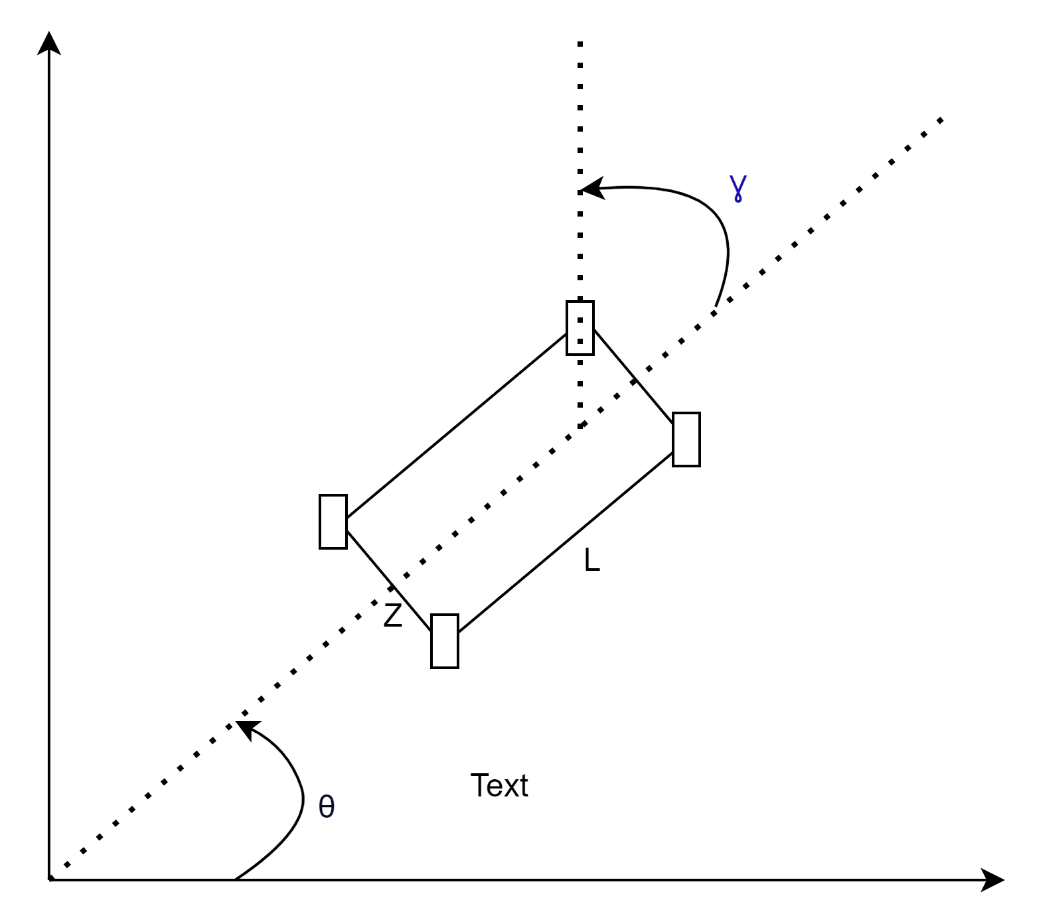
\includegraphics[width=0.6\textwidth]{img/diagrams/1schema_robo.png} 
    \caption{Schéma du robo.}
    \label{img-abc_dq}
\end{figure}


L'état du robot est caractérisé par sa position $(x, y)$ et son orientation $\theta$. Les expressions des vitesses linéaire $v$ et angulaire $W$ sont dérivées des équations dynamiques sur \ref{eq:eq_dyn_cartesian}. En coordonnées polaires, les dynamiques du système sont exprimées par \ref{eq:eq_dyn_polaire}.

\begin{align}
\begin{split}
    & \dot{x} = v \cdot cos(\theta) \\
    & \dot{y} = v \cdot sin(\theta)
    \label{eq:eq_dyn_cartesian}
\end{split}
\end{align}


\begin{align}
\begin{split}
    &\dot{\phi} = v \cdot cos(\alpha) \\
    &\dot{\beta} = v \cdot sin(\phi)/\rho \\
    &\dot{\alpha} = -v \cdot sin(\alpha)/\rho - W
    \label{eq:eq_dyn_polaire}
\end{split}
\end{align}


La commande du robot est régie par les équations \ref{eq:commande}, où $K_\rho$, $K_\alpha$, et $K_\beta$ sont des gains de contrôle ajustant la réponse en fonction des erreurs angulaires $\rho$, $\alpha$, et $\beta$. Ces équations forment l'épine dorsale du système de contrôle, indiquant la manière dont les vitesses linéaire et angulaire sont déterminées en fonction des erreurs de position et d'orientation.


\begin{align}
\begin{split}
    & v = K_{\rho} \cdot \rho \\
    & W = K_{\alpha} \cdot \alpha + K_{\beta} \cdot \beta
    \label{eq:commande}
\end{split}
\end{align}


\subsubsection{Validation du Cas A vers l’origine}


Nous avons ensuite enrichi notre modèle avec des angles additionnels, notamment l'angle $\beta$ défini entre l'axe reliant le point A à l'origine $(0,0)$ et l'axe des abscisses. L'incorporation de $\beta$, en conjonction avec $\rho$ (la distance euclidienne à l'origine) et $\alpha$ (l'angle entre la position actuelle et l'origine), augmente la finesse du modèle de contrôle.

\begin{figure}[!h]
    \centering
    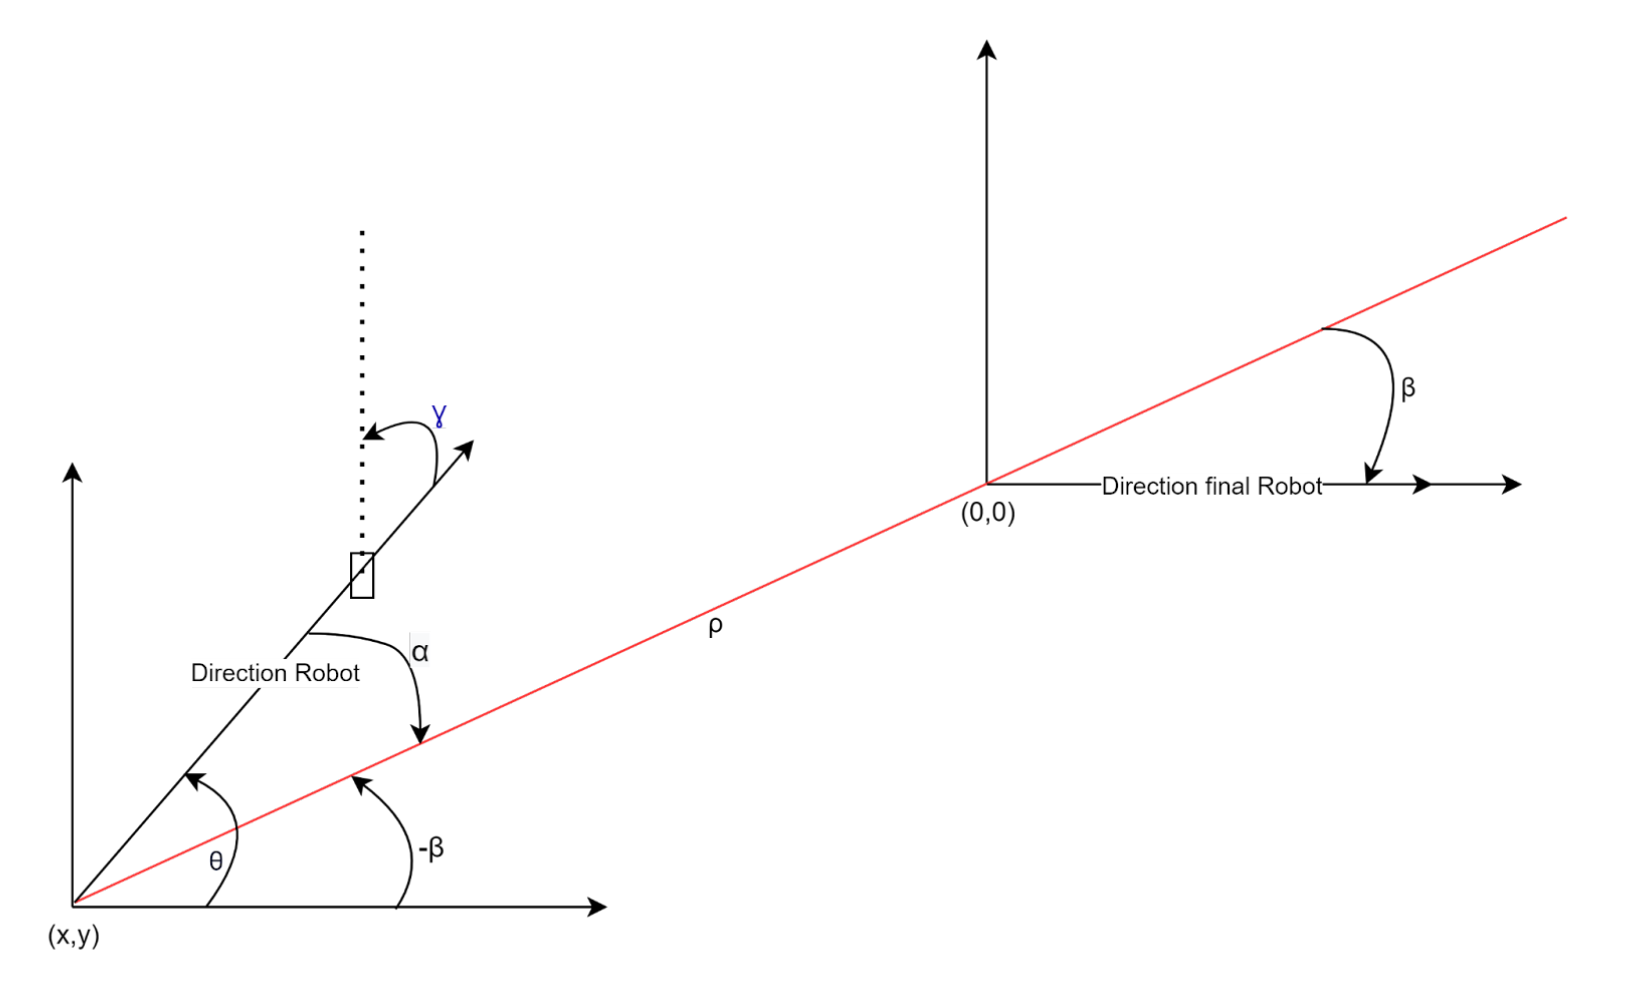
\includegraphics[width=1.0\textwidth]{img/diagrams/2schema_transformation.png} 
    \caption{Diagramme de Trajectoire du Robot - De l'Origine au Point A}
    \label{img-abc_dq}
\end{figure}
\FloatBarrier
Ce schéma nous donne les équations : 

\begin{align*}
\begin{split}
    & \rho = \sqrt{(x^2+y^2)} \\
    & \beta = -arctan\left( \frac{y}{x} \right) \\
    & \alpha = -(\theta + \beta)
\end{split}
\end{align*}


Pour identifier les gains optimaux $K_\rho$, $K_\alpha$, et $K_\beta$, des calculs basés sur des scénarios de navigation spécifiques sont nécessaires. Ces gains régulent la vitesse linéaire et angulaire en fonction des erreurs de position et d'orientation, ce qui est crucial pour diriger le robot du point A vers l'origine avec une orientation finale $\theta = 0$. Les équations établies permettent une modélisation précise des trajectoires et des corrections nécessaires.


Dans le cadre de l'analyse de stabilité, les équations différentielles qui décrivent les dynamiques du robot sont linéarisées autour d'un point d'équilibre. En calculant $\dot{\rho}$, $\dot{\beta}$ et $\dot{\alpha}$ et en remplaçant v et W par $K_\rho$ $\rho$ et $K_\alpha \alpha + K_\beta \beta$ respectivement, nous obtenons une matrice $A$ du système linéarisé. L'analyse de stabilité requiert de vérifier si toutes les valeurs propres de la matrice A ont des parties réelles négatives. Les conditions de stabilité, $K_\rho > 0$, $K_\beta < 0$, $K_\alpha > K_\rho$, assurent que les erreurs diminuent avec le temps, guidant le robot vers son état d'équilibre souhaité.


\subsubsection{Validation du Cas A vers B}


Enfin, pour compléter notre validation théorique, nous avons étendu le modèle pour permettre au robot de naviguer d'un point A à un point B, tout en ajustant sa trajectoire et son orientation pour une efficacité optimale. L'intégration de $\tilde{\beta}$ (l'écart angulaire entre la droite AB et l'orientation actuelle du robot) enrichit la capacité de contrôle du système, permettant une navigation précise et adaptée à des objectifs de positionnement et d'orientation spécifiques. Cette extension montre la flexibilité et la robustesse du modèle de contrôle, capable de s'adapter à diverses exigences de navigation dans des environnements dynamiques et changeants.


\begin{figure}[!h]
    \centering
    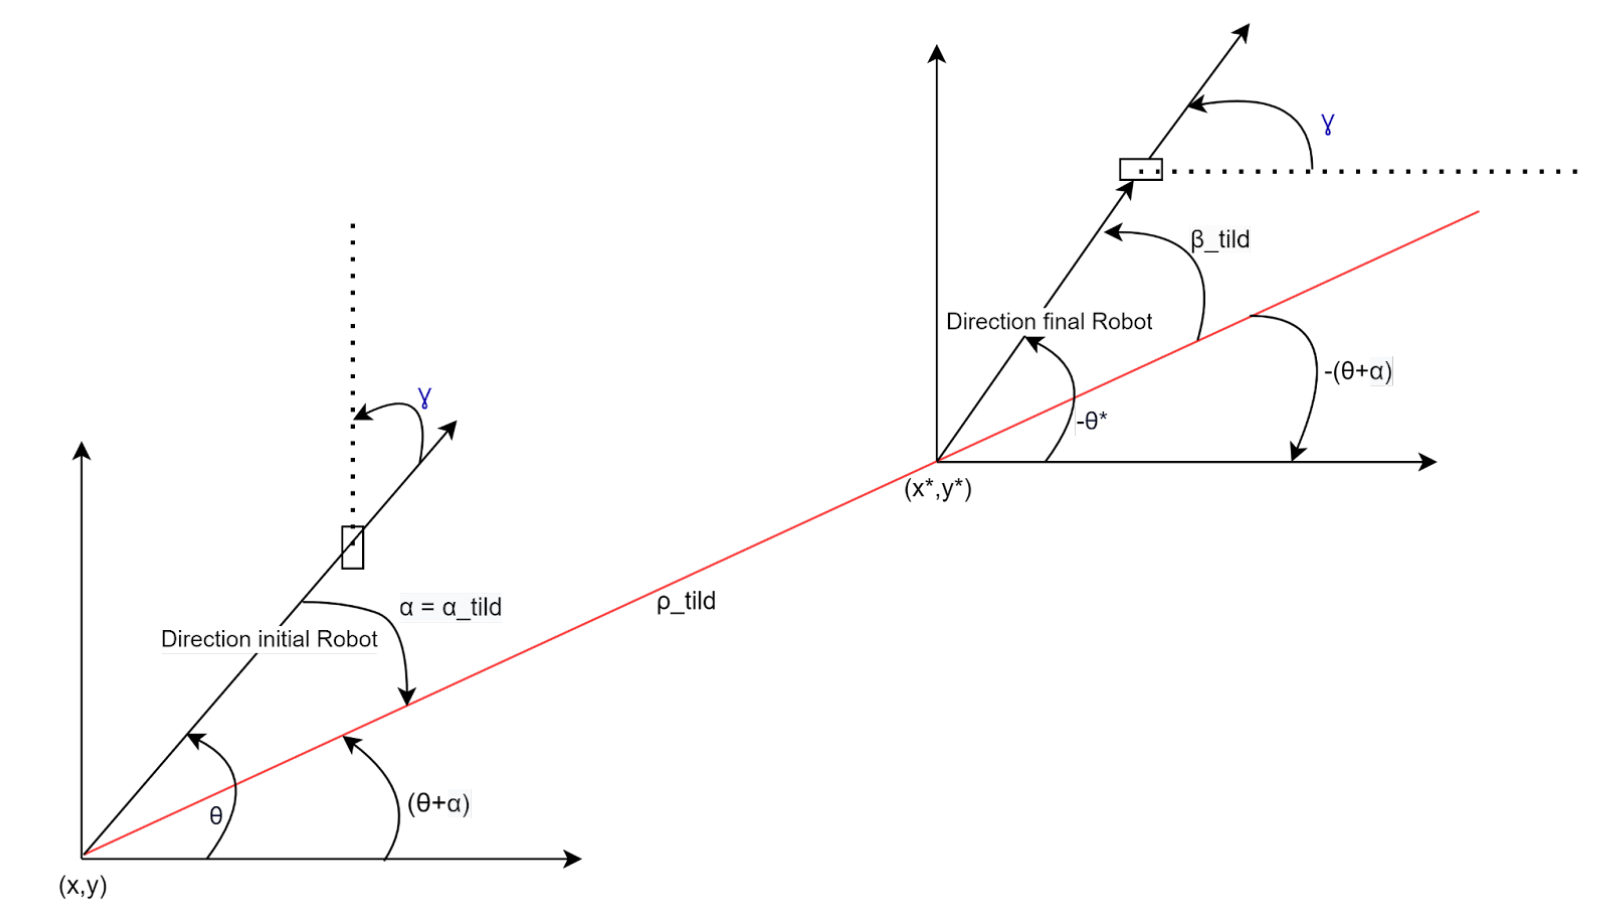
\includegraphics[width=1.0\textwidth]{img/diagrams/3schema_transformation2.png} 
    \caption{Diagramme de Trajectoire du Robot - Du Point A au Point B}
    \label{img-abc_dq}
\end{figure}


Le calcul des équations : 

\begin{align*}
\begin{split}
    \tilde{\rho} = \sqrt{{dx}^2 + {dy}^2} \\
    \tilde{\beta} = -arctan\left(\frac{dx}{dy}\right) - \theta^* \\
    \tilde{\alpha} = arctan\left(\frac{dx}{dy}\right) - \theta 
\end{split}
\end{align*}


sont essentiels pour déterminer respectivement la distance corrigée, l'écart angulaire corrigé par rapport à l'orientation finale souhaitée, et l'écart angulaire corrigé par rapport à l'orientation actuelle du robot.


\subsection{Validation en Simulation}



%Tous les fichiers slx et mlx sont disponibles sur le GitHub.


\subsubsection{Simulation du Cas A vers l’origine}

Cette première sous-partie décrit la simulation du robot se déplaçant du point A à l'origine $(0,0)$ tout en ajustant son orientation.

\textbf{Initialisation et Paramètres du Modèle :}

\begin{itemize}
    \item Définition du point de départ (A) : Configuré dans le fichier MLX.
    \item Réglage des Paramètres et Gains du Contrôleur : Nous avons fixé $K_\rho = 1$, $K_\beta = -1$, $K_\alpha = 5$, suite à une série de tests et conformément aux conditions établies précédemment.
    \item Modélisation de la Dynamique : Utilisation des équations de mouvement adaptées pour modéliser le comportement dynamique du robot.
\end{itemize}

\begin{figure}[!h]
    \centering
    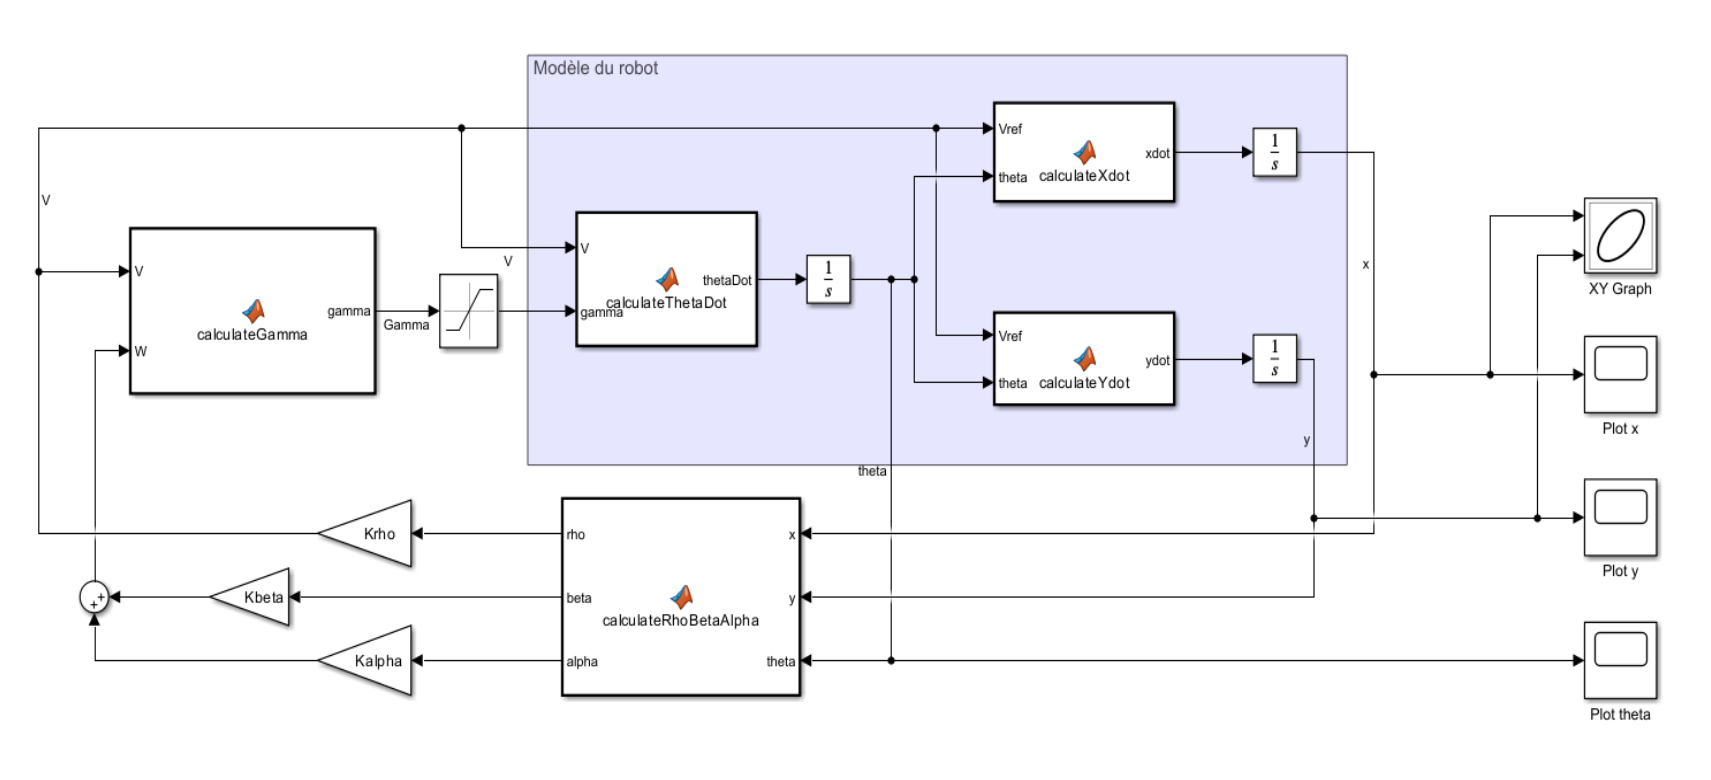
\includegraphics[width=1.0\textwidth]{img/diagrams/4modelisaiton_matlab.png} 
    \caption{Modèle Simulink de la dynamique du fonctionnement robot depuis un point A jusqu'à l'origine.}
    \label{img:simulink1}
\end{figure}

\textbf{Dynamique et Contrôle :}

\begin{itemize}
    \item Calculs MATLAB : Emploi de fonctions MATLAB pour déterminer $\gamma$, $\theta$, la vitesse linéaire ($v$) et la vitesse angulaire ($\omega$), intégrant les équations de mouvement pour le suivi de trajectoire.
    \item Test de Départ : Position initiale ($x_0 = -2$, $y_0 = -4$, $\theta_0 = -\pi$).
\end{itemize}



% -----------------

%On définit un point de départ A dans le ficher mlx. 

% Configuration des paramètres du robot et des gains du contrôleur ($K_rho$, $K_\beta$, $K_\alpha$) à optimiser. On a choisi $K_\rho = 1$; $K_\beta = -1$; $K_\alpha = 5$;  après une série de test et les conditions données dans la partie précédente.
% Modélisation de la dynamique du robot avec les équations de mouvement adaptées.


% Utilisation de fonctions MATLAB pour le calcul de $\gamma$, $\theta$, vitesse linéaire ($v$) et vitesse angulaire ($\omega$).
% Intégration des équations de mouvement pour le suivi de la trajectoire.
% Suggestion d'image : Diagramme du modèle de robot avec angles et vecteurs de vitesse.

% Résultats et Ajustements :

% Observation de la trajectoire du robot et ajustement des gains du contrôleur pour assurer une navigation précise vers l'origine.
% Analyse des performances et identification des améliorations nécessaires.
% Suggestion d'image : Graphiques des trajectoires simulées et des réglages de gains.

% -----------------

\textbf{Simulation du Cas A vers B}


Cette partie traite de la simulation plus complexe où le robot se déplace du point A ($x_a$, $y_a$, $\theta_a$) vers un point B ($x^*$, $y^*$, $\thet^*$) prédéfini, avec une orientation finale spécifique.


Mise à Jour des Conditions Initiales :

\begin{itemize}
    \item Inclusion de la Position et Orientation Finale pour le Point B : Modification des conditions initiales pour intégrer la destination et l'orientation de B.
    \item Adaptation des Fonctions de Calcul : Mise à jour des fonctions pour refléter la nouvelle destination et orientation.
\end{itemize}

\FloatBarrier

\begin{figure}[!h]
    \centering
    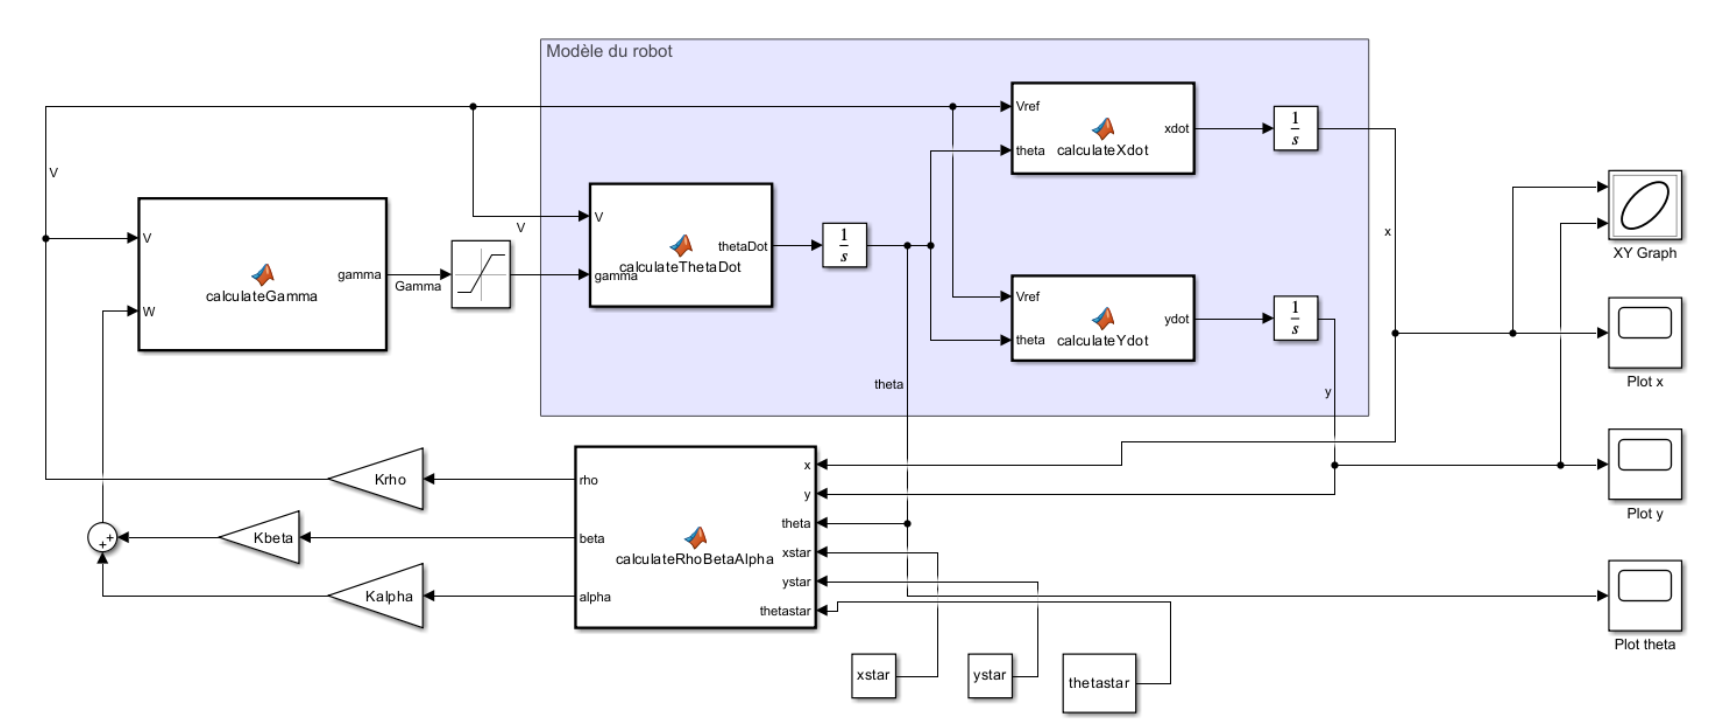
\includegraphics[width=1.0\textwidth]{img/diagrams/6} 
    \caption{Modèle Simulink de la dynamique du fonctionnement robot d’un point A à un point B}
    \label{img:simulink2}
\end{figure}

Test et Ajustements :
\begin{itemize}
    \item Modification des erreurs $\rho$, $\beta$, $\alpha$: Ajustement pour correspondre aux exigences de la nouvelle trajectoire.
    \item Ajustement des Gains du Contrôleur : Réglage en fonction des nouvelles conditions.
    \item Nouveau Test : Avec les valeurs ($x_a = 10$, $y_a = -3$, $\theta_a = -pi/4$ pour A et $x^* = 4$, $y^* = -1$, $\theta^* = 0$ pour B).
\end{itemize}



% Configuration pour le Point B :

% Mise à jour des conditions initiales pour inclure la position et l'orientation finale souhaitées pour le point B.
% Adaptation des fonctions de calcul pour tenir compte de la nouvelle destination et orientation.
% Suggestion d'image : Capture d'écran des paramètres mis à jour dans MATLAB.

% Adaptation de la Logique de Contrôle :

% Modification des calculs des erreurs rho, beta, alpha pour correspondre aux nouvelles exigences de la trajectoire.
% Ajustement des gains du contrôleur en fonction des nouvelles conditions.
% Suggestion d'image : Schéma illustrant la nouvelle configuration de trajectoire et d'orientation.

% Analyse de la Trajectoire et Optimisation :

% Tests de la simulation dans divers scénarios pour évaluer la robustesse du contrôleur.
% Observation des changements de comportement du robot et ajustements fins pour atteindre les objectifs de position et d'orientation.
% Suggestion d'image : Visualisations des trajectoires du robot de A vers B dans différents tests.


% Validation Expérimentale


\section{Étape 2 : Supervision du Véhicule
Système de Supervision}

\subsection{Test des fonctions du module pylimo}

Pour commander le robot, d'abord, les modules de la librairie pylimo \cite{pylimo}, qui sont responsables de donner les commandes et de récupérer les informations pertinentes du robot, ont été testés. Des scripts ont été générés pour comprendre comment l'extraction des données des capteurs du robot se fait et comment appliquer les commandes à la voiture.

Les données suivantes ont été identifiées comme étant capturées par le robot :

\begin{itemize}
    \item \textit{vitesse linéaire}, type \textit{float}
    \item \textit{vitesse angulaire}, type \textit{float}
    \item \textit{angle de braquage}, type \textit{float}
    \item \textit{vitesse latérale}, type \textit{float}
    \item \textit{mode de contrôle}, type \textit{int}
    \item \textit{tension de la batterie}, type \textit{float}
    \item \textit{code d'erreur}, type \textit{int}
    \item \textit{données de l'accéléromètre}, type \textit{tuple}
    \item \textit{données du gyroscope}, type \textit{tuple}
\end{itemize}

Ensuite, les modules responsables du mouvement du robot ont été testés dans une boucle, en donnant une série d'instructions au robot pour le mouvement à travers la méthode \textit{SetMotionCommand}, modifiant la vitesse linéaire du robot et l'angle des roues. En testant le comportement de la librairie Python pylimo du robot et en lisant la documentation du robot sur le GitHub d'Agilex Robotics \cite{LimoDocGitHub}, il a été possible de découvrir le comportement du robot en utilisant les modules de mouvement. Une caractéristique importante qui a été remarquée est que l'angle maximal des roues de 30° est équivalent à une commande de 0.30.

\subsection{Codage du package limo\_controller}

À partir des informations acquises et de l'étude des modules et des outils à utiliser, incluant ROS2, il a été possible de coder un algorithme Python responsable de générer un nœud qui récupérait les informations de vitesse linéaire et l'angle des roues sur des topics.

Ce nœud fait partie du module \textit{limo\_controller}, qui a été créé pour regrouper tous les nœuds développés dans le projet. À partir de ce package, il a été possible de diviser les tâches de contrôle du robot en différents nœuds.

Ainsi, des nœuds ont été créés pour générer le contrôle du robot, un nœud pour appliquer ce contrôle, et des nœuds de surveillance. En termes de nœuds de contrôle, trois ont été créés : un nœud pour le contrôle du robot via le clavier, un nœud de contrôle via une interface tkinter en cliquant sur des flèches à l'écran, et le troisième nœud responsable du contrôle automatique du véhicule, simulant l'environnement où il se déplacerait, permettant de définir un point de départ et d'arrivée, et où le véhicule tracerait sa trajectoire.

Des fonctions auxiliaires ont également été développées pour tester les fonctionnalités implémentées dans les nœuds. De plus, dans les nœuds utilisant une interface graphique, la bibliothèque Python Tkinter a été utilisée.


\subsection{Développement de l'interface de commande automatique}

Pour l'interface de commande automatique, une image d'arrière-plan a été créée afin de reproduire l'environnement dans lequel le robot serait testé. Cette image a été conçue en utilisant la plateforme draw.io \cite{diagramsnet}, comme le montre l'image \label{imgxx}.

\begin{figure}[!h]
    \centering
    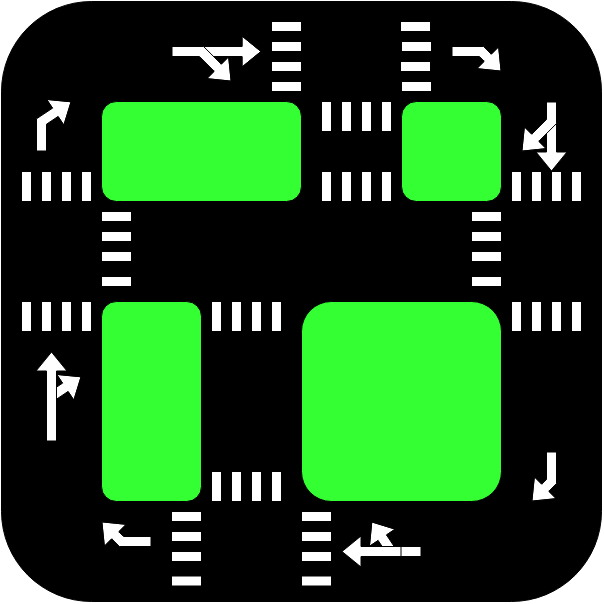
\includegraphics[width=0.6\textwidth]{img/background/background.png} 
    \caption{Image de fond créée sur la plateforme draw.io}
    \label{imgxx}
\end{figure}

L'objectif final était de permettre de sélectionner un point de départ et d'arrivée et de faire en sorte que le nœud réalise une animation du véhicule parcourant le chemin sur l'écran, tout en publiant la commande de vitesse linéaire et l'angle des roues sur les topics correspondants. Ces commandes seraient ensuite lues par le nœud qui applique le commandement, par une publication au topic.

Pour interpréter le chemin, un algorithme a été développé pour lire l'image de l'environnement et définir les points où l'utilisateur ne peut pas cliquer (régions blanches), les points correspondant à la route où l'utilisateur peut cliquer (points noirs ou verts) et les points correspondant à la trajectoire que le véhicule peut emprunter. Une nouvelle image a été créée en retirant les éléments non pertinents de l'environnement, qui a ensuite été analysée par une fonction auxiliaire pour générer la matrice indiquant ces éléments de l'environnement (image \ref{AAA}).

\FloatBarrier
\begin{figure}[!h]
    \centering
    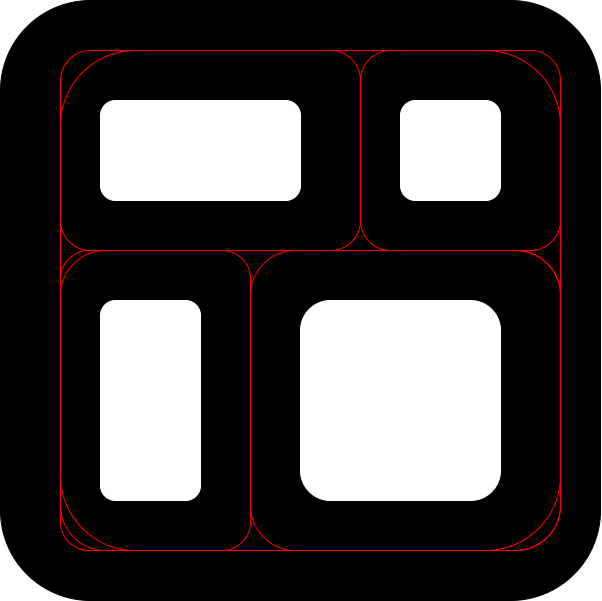
\includegraphics[width=0.6\textwidth]{img/background/trace_track.png} 
    \caption{Image créée pour extraire des informations sur l'environnement.}
    \label{AAA}
\end{figure}

Afin d'améliorer la trajectoire pouvant être suivie par le véhicule, une version améliorée de la trajectoire a été dessinée à la main à partir de l'image précédente \ref{imgff}. 

\begin{figure}[!h]
    \centering
    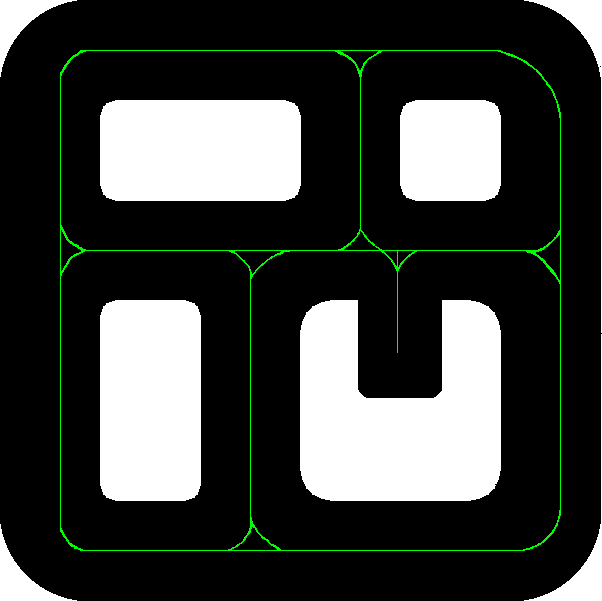
\includegraphics[width=0.6\textwidth]{img/background/track_improove.png} 
    \caption{Image améliorée pour extraire des informations sur l'environnement.}
    \label{imgff}
\end{figure}



Pour calculer le chemin le plus court possible entre le point de départ choisi et le point d'arrivée, l'algorithme de recherche A* (A star) a été utilisé. L'algorithme de recherche A* est une technique de recherche de chemin qui trouve le chemin le plus court entre deux points en utilisant une heuristique pour minimiser le coût total estimé du chemin.

La fonction appliquant l'algorithme de recherche A* a été validée à l'aide d'une fonction auxiliaire.





